\documentclass[11pt]{article}

\usepackage[a4paper, margin=2cm, top=1.9cm, bottom=1.9cm]{geometry}
\usepackage[utf8]{inputenc}
\usepackage[T1]{fontenc}
\usepackage[brazilian]{babel}
\usepackage{enumitem}
\usepackage{graphicx}
\usepackage{xcolor}
\usepackage{titlesec}
\usepackage[hidelinks]{hyperref}

\setlength{\parindent}{0pt}
\setlength{\parskip}{5pt}
\pagestyle{empty}
\linespread{1.07}

\definecolor{accent}{HTML}{1F3864}

\newcommand{\topico}[1]{%
  \vspace{7pt}
  {\Large\bfseries\color{accent} #1}\par
  \vspace{2pt}
}

\setlist[itemize]{itemsep=3pt, parsep=0pt, topsep=3pt, partopsep=0pt, leftmargin=1.5em}
\setlist[enumerate]{itemsep=3pt, parsep=0pt, topsep=3pt, partopsep=0pt, leftmargin=1.7em}

\begin{document}

%================= PÁGINA 1 =================

\begin{center}
  {\huge\bfseries\color{accent} Guia de Sucesso nas Disciplinas de Exatas}\\[4pt]
\end{center}
\vspace{4pt}

\noindent Este guia foi escrito para você que está iniciando um curso de engenharia ou matemática e vai enfrentar, já no primeiro período, disciplinas como Cálculo, Geometria Analítica e Física. Sei que a base trazida do ensino médio nem sempre é a ideal, e isso não é culpa sua nem motivo para desanimar. O que se segue são princípios e métodos práticos, testados, para você estudar com inteligência, manter a disciplina e construir resultados consistentes ao longo da sua trajetória acadêmica.

\topico{1. Identidade e propósito}

Entrar na universidade é muito mais do que escolher um curso; é iniciar uma jornada de construção pessoal. Nem sempre a primeira escolha será a perfeita, e isso faz parte da vida. O importante é não caminhar sem saber quem você é e por que está fazendo o que faz.

Quando as provas ficarem difíceis, o cansaço aparecer e as dúvidas surgirem, será o seu propósito que dará sentido ao esforço. E será a sua identidade que impedirá que você desista diante das dificuldades.

Se, ao longo do caminho, você descobrir que escolheu o curso errado, tenha coragem para reavaliar a direção. Mas não abandone seus sonhos por causa dos primeiros obstáculos. Antes de tomar qualquer decisão, reflita: você está desistindo porque encontrou o caminho errado ou porque o caminho ficou difícil?

Quem conhece sua identidade e vive com propósito segue firme até atingir seus objetivos.

\topico{2. Disciplina}
Disciplina é o que garante energia, foco e saúde durante a semana — fundamental para o desempenho nos estudos e para reduzir a chance de imprevistos, como adoecer justo em dia de prova.
\begin{itemize}
  \item Alimente-se bem: priorize legumes, salada e proteína.
  \item Durma cedo e busque entre 7 e 9 horas de sono por noite.
  \item Exercite-se ao menos 3x por semana (corrida e/ou musculação são boas opções).
  \item Estude diariamente, com consistência, mesmo que por poucas horas.
  \item Evite distrações: perceba o que rouba sua atenção e afaste-se disso durante o estudo.
\end{itemize}

\topico{3. Construa uma base forte}
Antes de erguer um edifício, é preciso garantir que seus alicerces sejam sólidos. Na universidade acontece o mesmo: disciplinas como Cálculo exigem uma base consistente em matemática básica. Se essa base tem lacunas, não veja isso como motivo para desistir, mas como um chamado para fortalecê-la. Dedique tempo aos pré-requisitos, revise conteúdos sempre que necessário e não tenha vergonha de voltar alguns passos para avançar com segurança. O aprendizado em exatas é cumulativo: cada novo conceito se apoia no anterior. Investir na sua base hoje é o que vai permitir resultados cada vez melhores ao longo de toda a sua trajetória acadêmica.

\topico{4. Como estudar acompanhando as aulas}
\begin{itemize}
  \item Anote apenas os pontos essenciais, para não perder a atenção durante a aula.
  \item Pergunte sempre que surgir uma dúvida — não a leve para casa sem necessidade.
  \item No mesmo dia, após a aula, revise o conteúdo e refaça os exemplos resolvidos em sala.
  \item Tenha um livro de apoio indicado pelo professor para estudar por conta própria.
\end{itemize}

\newpage
%================= PÁGINA 2 =================

\topico{5. Caderno de guerra}
Aqui vai uma maneira eficiente de estudar qualquer assunto de matemática em profundidade. Você vai precisar de um livro-texto e de um caderno (de guerra) para registrar tudo o que julgar importante no seu aprendizado. É um caderno que você deve revisitar sempre que a memória começar a lhe trair — assim você retém conhecimento e habilidades a longo prazo. Siga os passos abaixo, na ordem.

\begin{enumerate}
  \item[\textbf{1.}] \textbf{Leitura do conteúdo} --- ao começar um novo capítulo ou seção do livro, repita os passos abaixo antes de seguir para o próximo:
  \begin{enumerate}
    \item[\textbf{1.a}] Verifique detalhes omitidos nas explicações, exemplos e demonstrações.
    \item[\textbf{1.b}] Reescreva, com suas próprias palavras, as definições e teoremas.
    \item[\textbf{1.c}] Refaça as demonstrações mais simples de memória, até onde conseguir.
  \end{enumerate}
  \item[\textbf{2.}] \textbf{Seleção de exercícios} --- escolha exercícios que satisfaçam um dos critérios abaixo:
  \begin{enumerate}
    \item[\textbf{2.a}] A primeira ideia de ataque não é óbvia.
    \item[\textbf{2.b}] Exige a construção de algum objeto matemático (função, matriz, vetor etc.), em particular encontrar exemplos ou contraexemplos.
  \end{enumerate}
  \item[\textbf{3.}] \textbf{Estratégia de ataque a exercícios:}
  \begin{enumerate}
    \item[\textbf{3.a}] Entenda o enunciado, com todas as hipóteses e o que se pede.
    \item[\textbf{3.b}] Elabore um plano de ataque.
    \item[\textbf{3.c}] Se o plano falhar, tente outro. Repita esse processo por até uma hora (tempo-limite).
  \end{enumerate}
  \emph{Obs.: se não resolver o exercício, anote o ponto (ou motivo) onde travou e, se conseguir, deixe registrada a primeira pista que pareça útil. Retorne à questão depois — pode ser dias ou até semanas.}
  \item[\textbf{4.}] \textbf{Crie exercícios para desenvolver criatividade} --- recrie exercícios semelhantes aos que você já resolveu, alterando hipóteses, construindo funções, trocando constantes etc. Assim você passa a dominar o conteúdo de verdade.
\end{enumerate}

Sei que nem sempre haverá tempo para cumprir todos esses pontos à risca. Mas eles ficam como referência para quando você quiser dominar um conteúdo por completo.

\vspace{4pt}

\begin{center}
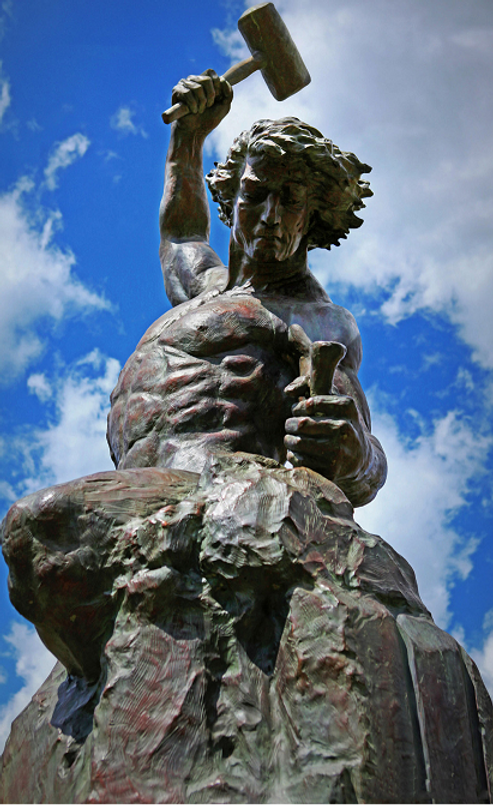
\includegraphics[width=4.1cm]{escultor.png}
\end{center}

\vspace{3pt}
\begin{center}
{\large\itshape ``O homem não pode reconstruir-se sem sofrimento, pois ele é ao mesmo tempo o mármore e o escultor.''}\\[3pt]
{\large --- Alexis Carrel}
\end{center}

\end{document}
